\subsection{Соединения фосфора, способы получения, химическое поведение, электронное и геометрическое строение молекул}
\textbf{Строение}

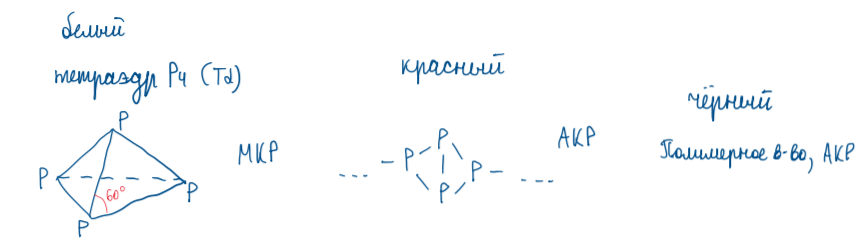
\includegraphics{images/9v1.png}

\subsubsection*{$PH_3$ и фосфиды}

\textbf{Получение}

$$MeP + H2O \rightarrow Me(OH)_x + PH_3$$
$$P + MeOH + H_2O \rightarrow PH_3 + MeH_2PO_2$$
$$[PH_4]R + MeOH \rightarrow MeR + PH_3 + H_2O$$
$$Me + P \rightarrow MeP^{3-}$$

\textbf{Химические свойства}

1) Разложение

$$PH_3 \rightarrow P + H_2$$

2) Слабые основные свойства

$$PH_3 + HI \rightarrow [PH_4]^+I^-$$

3) Сильный восстановитель

$$PH_3 + O_2 \rightarrow HPO_3 + H_2O$$
$$PH_3 + MnO_4 + H^+ \rightarrow PO_4^{3-}+...$$

4) Фосфиды  гидролиз  и горение

$$MeP + O_2 \rightarrow MeO + P_2O_5$$
$$MeP + H2O \rightarrow Me(OH)_x + PH_3$$

\textbf{Строение}

Слабее поляризованы связи $P-H$, чем у $NH_3 \Rightarrow$ слабее как основание;\\
Активность НЭП $P (3s^2)$ ниже НЭП $N (2s^2)$, нет водородных связей

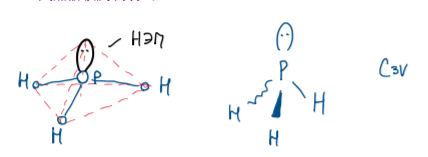
\includegraphics{images/9v2.png}

\subsubsection*{Галогениды}

Есть в +3, и в +5, кроме $PI_5$

\textbf{Получение}

1) Прямым синтезом из простых веществ при разных условиях и соотношениях

$$2P + 5Cl_2 \rightarrow 2PCl_5$$
$$2P + 2Cl_2 \rightarrow 2PCl_3$$

$$PCl_x \xrightarrow{CaF_2/ZnF_2/AsF_3} PF_x(x=3,5)$$

\textbf{Химические свойства}

1) $PF_3$ - яд, не взаимодействует с $H_2O$, прочные комплексы с d-металлами

2) $PX_3$ - гигроскопичны (x = Cl, Br, I)

$$PX_3 + H_2O \rightarrow H_3PO_3 + HX$$

3) $PX_3$ - донорные свойства (x=Cl,Br,I)

4) $PX_5$ - галогенангидриды

$$PX_5 + H_2O \rightarrow H_3PO_4 + HX$$
$$POCl_3 + H_2O \rightarrow H_3PO_4 + HCl$$

5) Донорные свойства

$$PCl_5 + BCl_3 \rightarrow [PCl_4]^+[BCl_4]^-$$
$$PCl_5 + KF \xrightarrow{\approx 200^{\circ}} K[PF_6] + KCl$$
$$PCl_5 + NH_4Cl \rightarrow (PNCl_2)_3$$
$$PCl_5 + P_3O_10 \xrightarrow{150^{\circ}} POCl_3$$

6) С органическими веществами

$$PCl_5 + RCOOH \xrightarrow{60^{\circ}} RCOCl + POCl_3 + H_2O$$
$$PCl_5 + ROH \rightarrow RCl + POCl_3 + HCl$$

\textbf{Электронное и геометрическое строение}

$PF_5$ - молекулярный\\
$PCl_5$ - молекулярный в газовой фазе, в твердой фазе $[PCl_4]^{+}[PCl_6]^-$\\
$PBr_5$ в твердой фазе $[PBr_4][Br]^-$

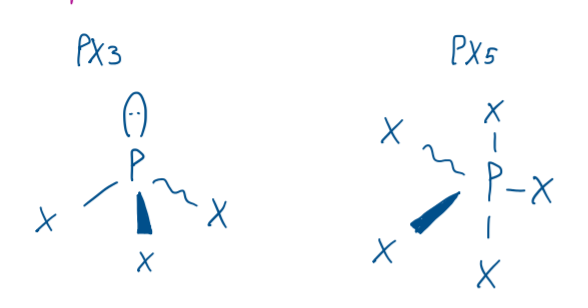
\includegraphics{images/9v3.png}

Диаграмма МО на примере $PF_5$ (рассматриваем p-орбитали F, направленные к P)

%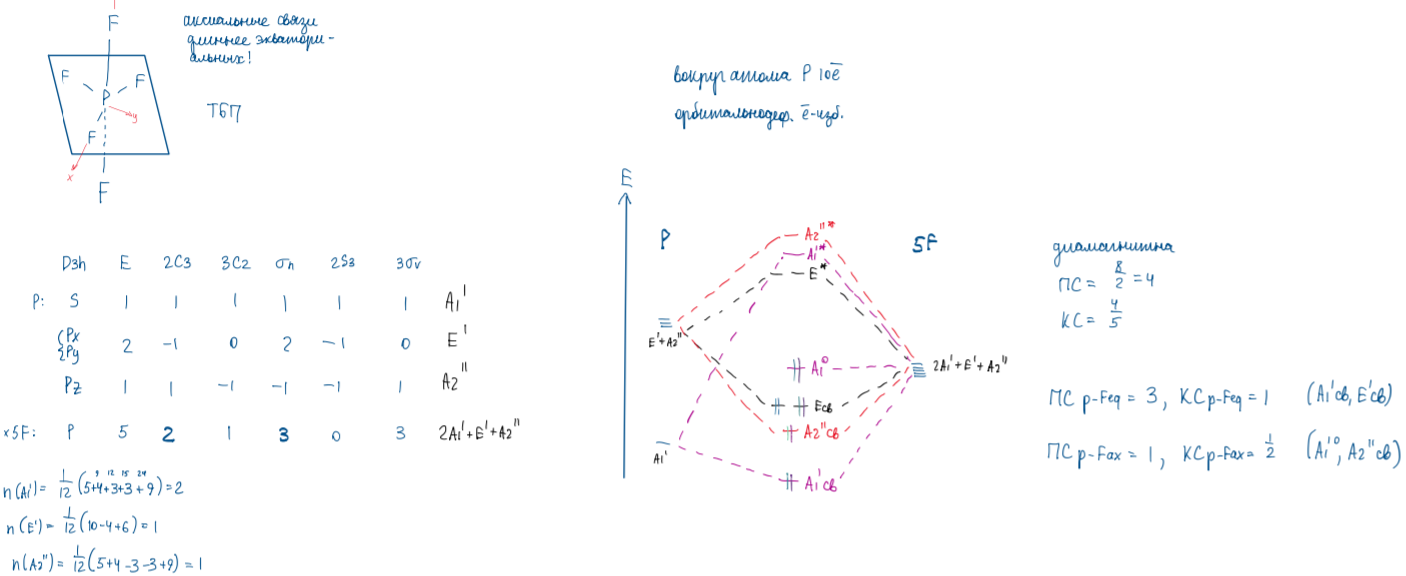
\includegraphics[scale=0.75]{images/9v4.png}

Аксиальные связи менее прочные и более длинные

\subsubsection*{$P_2O_3 \leftrightarrow P_4O_6$}

\textbf{Получение}

$$P + O_2 \rightarrow P_2O_3$$
$$P_4 + N_2O \xrightarrow{550-635^{\circ}} P_4O_6 + N_2$$
$$P_4 + CO_2 \xrightarrow{650^{\circ}} P_4O_6 + CO$$
$$P_4 + P_4O_{10} \xrightarrow{50^{\circ}}$$

\textbf{Химические свойства}

1) Ангидрид фосфористой кислоты

$$P_4O_6 + H_2O \xrightarrow{holod} H_3PO_3$$
$$P_4O_6 + H_2O \xrightarrow{gor} P\downarrow + H_3PO_4 + PH_3\uparrow$$

2) Сильный восстановитель

$$P_4O_6 + O_2 \xrightarrow{50-120^{\circ}} P_4O_10$$
$$P_4O_6 + Cl_2  \rightarrow POCl_3 + O_2$$
$$P_4O_6 + S \rightarrow P_4S_6 + SO_2$$

\textbf{Строение}

В парах состоит из молекул $P_4O_6$\\
Тетраэдр из P, и на каждом ребре O

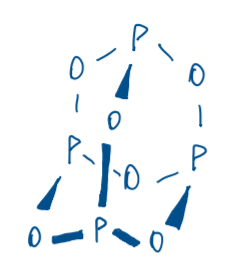
\includegraphics{images/9v5.png}

\subsubsection*{$P_2O_5 \leftrightarrow P_4O_{10}$}

\textbf{Получение}

$$ P + O_2 \rightarrow P_4O_{10}$$

Разложение при сильном нагревании:

$$P_4O_{10} \rightarrow P_4O_6 + O_2$$

Ангидрид фосфорной кислоты

$$P_4O_{10} + H_2O \rightarrow H_3PO_4$$

Все свойства кислотных оксидов

Сильное водоотнимающее средство 

$$P_4O_{10} + HNO_3 \rightarrow HPO_3 + N_2O_5$$
$$P_4O_{10} + HClO_4 \rightarrow HPO_3 + Cl_2O_7$$

С RCOOH

$$P_4O_{10} + RCOOH \rightarrow H_3PO_4 + (RCO)_2O$$

\textbf{Строение}

В парах состоит из молекул $P_4O_{10}$\\
Кристаллическое состояние - две метастабильные модификации:

- Гексагональная н-форма ($P_4O_{10}$ 4 группы в виде тетраэдра)

-Орторомбическая о-форма (химически менее активны, полимерные структуры из тетраэдров $PO_4$)

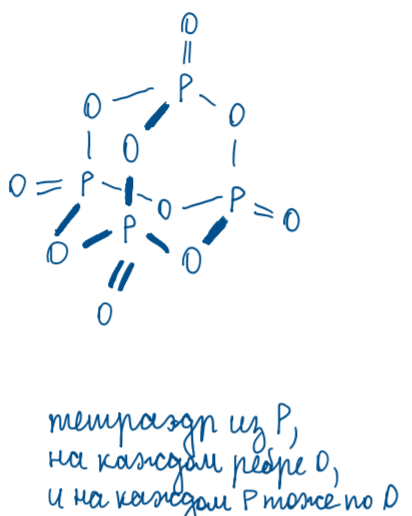
\includegraphics{images/9v6.png}

\subsubsection*{$HPF_6$}

\textbf{Получение}

$$H_3PO_4 + HF_{konc} \rightarrow HPF_6 + H_2O$$

\textbf{Химические свойства}

1) Существуют только в растворе

$$HPF_6 \leftrightarrows H^+ + PF_6^-$$

2) Не окислитель, не коррдинирующий ион

3) Соли растворимы в воде

\textbf{Строение}

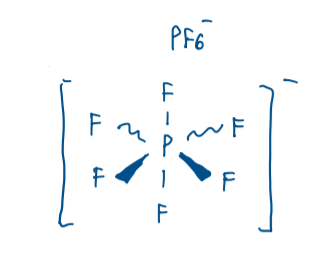
\includegraphics{images/9v7.png}

\subsubsection*{$H_3PO_2$ - фосфорноватистая}

\textbf{Получение}

$$Ba(H_2PO_2)_2 + H_2SO_4 \rightarrow H_3PO_2 + BaSO_4 \downarrow$$

\textbf{Химические свойства}

1) Сильная одноосновная кислота

$$H_3PO_2 \leftrightarrows H^+ + H_2PO_2^-$$

2) Диспропорционирование 

$$H_3PO_2 \rightarrow PH_3 + H_3PO_4$$

3) Очень сильный окислитель

$$H_3PO_2 + FeCl_3 + H_2O \rightarrow H_3PO_4 + FeCl_2 + HCl$$
$$NaH_2PO_2 + AgNO_3 + H_2O \rightarrow NaNO_3 + Ag + H_3PO-4 + HNO_3$$
4) Соли - гипофосфиты, хорошо растворимы в воде

\textbf{Строение}

$H(PH_2O_2)$
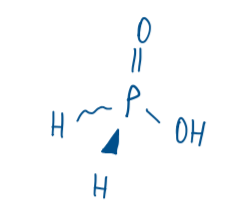
\includegraphics{images/9v8.png}

\subsubsection*{$H_3PO_3$ - фосфористая}

\textbf{Получение}

$$PCl_3 + H_2O \rightarrow H_3PO_3 + HCl$$
$$P_2O_3 + H_2O \rightarrow H_3PO_3$$
$$K_2HPO_3 + HCl \rightarrow KCl + H_3PO_3$$

\textbf{Химические свойства}

1) Двухосновная кислота средней силы, соли фосфины

2) Диспропорционирование

$$H_3PO_3 \rightarrow PH_3 + H_3PO_4$$
$$H_3PO_3 + O_2 \rightarrow H_4P_2O_6 + H_2O$$

3) Восстановительные свойства

$$H_3PO_3 + HgCl_2 + H_2O \rightarrow H_3PO_4 + Hg + HCl$$
\\
\textbf{Строение}

$H_2(PHO_3)$
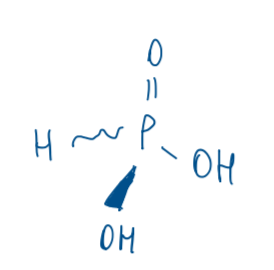
\includegraphics{images/9v9.png}

\subsubsection*{$H_4P_2O_6$ - фосфорноватая}

\textbf{Получение}

$$H_3PO_3 + O_2 \rightarrow H_4P_2O_6 + H_2O$$
$$Pb_2P_2O_6 + H_2S \rightarrow PbS + H_4P_2O_6$$

\textbf{Химические свойства}

1) Четырехосновная кислота, соли - фосфонаты, все плохо растворимы

$$H_4P_2O_6 \xrightarrow{73^{\circ}} H_3PO_3+ HPO_3$$
$$H_4P_2O_6 + H_2O \xrightarrow{25^{\circ}} H_3PO_3 + H_3PO_4$$

2) Восстановитель

$$H_4P_2O_6 + KMnO_4 + H_2SO_4 + H_2O \rightarrow K_2SO_4 + MnSO_4+ H_3PO_4$$

\textbf{Строение}

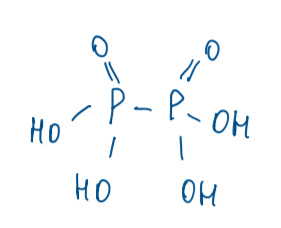
\includegraphics{images/9v10.png}

\subsubsection*{$H_3PO_4$ - ортофосфорная}

\textbf{Получение}

1) В лаборатории
$$P_2O_5 + H_2O \rightarrow H_3PO_4$$
$$P + HNO_{3(razb)} + H_2O \rightarrow H_3PO_4 + NO$$

2) В промышленности

$$Ca_3(PO_4)_2 + H_2SO_{4(konc)} \rightarrow  CaSO_4 + H_3PO_4$$

\textbf{Химические свойства}

1) Кислота средней силы трехосновная ( по 2 и 3 ступеням даже слабая)

$H_2PO_4^-$ - все соли растворимы\\
$HPO_4^{2-}$ - растворими только соли щелочных металлом, кроме Li\\
$PO_3^{3-}$ - то же самое

$$H_3PO_4 \rightarrow H_4P_2O_7 + H_2O$$

2) Не окислитель

3) Качественные реакции:

$$3Ag^+ + PO_4^{2-} \rightarrow Ag_3PO_4\downarrow$$

$$(NH_4)_6Mo_7O_24 + HNO_3 + H_3PO_3 \rightarrow (NH_4)_3[PMo_12O_40]\cdot 3H_2O\downarrow + NH_4NO_3 + H_2O$$

\textbf{Строение}

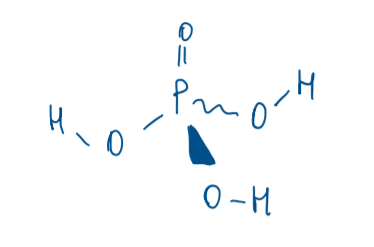
\includegraphics{images/9v11.png}

\subsubsection*{$H_4P_2O_7$ - пирофосфорная}

\textbf{Получение}

$$H_3PO_4 \xrightarrow[-H_2O]{250^{\circ}} H_4P_2O_7$$
$$H_3PO_4 + P_4O_{10} \xrightarrow{100^{\circ}} H_4P_2O_7$$

\textbf{Химические свойства}

1) Четырехосновная кислота (сильнее $H_4P_2O_6$)

$$H_4P_2O_7 \xrightarrow{300^{\circ}} HPO_3 + H_2O$$
$$H_4P_2O_7 + H_2O \xrightarrow{100^{\circ}, H^+} H_3PO_4$$
$$H_4P_2O_7 + AgNO_3 \rightarrow HNO_3 + Ag_4P_2O_7$$

\textbf{Строение}

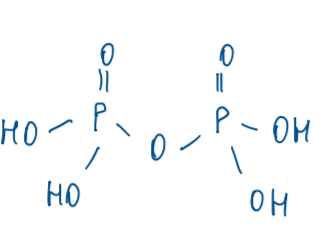
\includegraphics{images/9v12.png}

\subsubsection*{$(HPO_3)_n$ (n=3...8) - метафосфорная}

\textbf{Получение}

$$H_4P_2O_7 \xrightarrow{300^{\circ}} HPO_3 + H_2O$$
$$P_4O_10 + H_2O \rightarrow HPO_3$$

\textbf{Химические свойства}

1) Одноосновная кислота, хорошо растворима в воде

$$HPO_3 + H_2O \rightarrow H_3PO_4$$
$$Ca(PO_4)_2 + CaO \rightarrow Ca_3(PO_3)_2$$

\textbf{Строение}

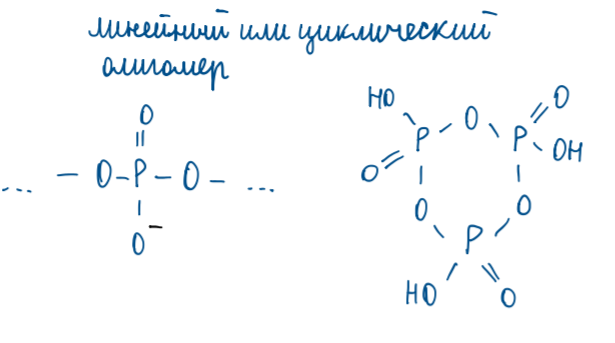
\includegraphics{images/9v13.png}
